\section{Типы галактик, эволюция галактик}

\subsection{Типы галактик}

Галактики согласно классификации Хаббла делятся на эллиптические (E), спиральные (S) и неправильные (Irr). Примеры красивых картинок можно найти на рисунке \ref{fig:16_galaxy_types}.

\begin{figure}[H]
	\centering
	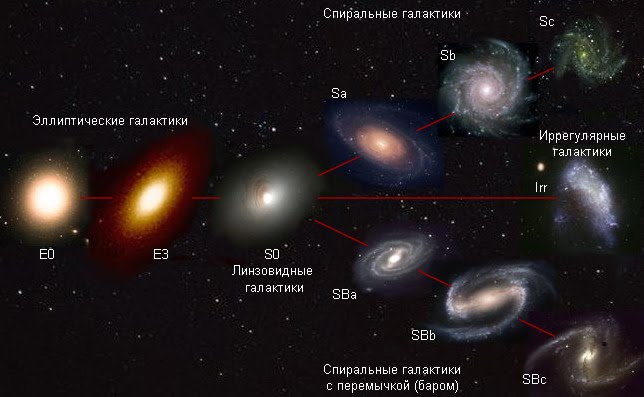
\includegraphics[width=0.9\linewidth]{16_galaxy_types}
	\caption{Типы галактик: эллиптические (E), спиральные (S) и неправильные (Irr)}
	\label{fig:16_galaxy_types}
\end{figure}

\subsubsection{Эллиптические галактики}

Эллиптические галактики имеют эллиптическую форму и характеризуются равномерной яркостью, которая постепенно убывает от края к центру.

Форма галактик данного типа варьируется от практически совершенно круглой, до сплюснутого эллипса. Соответственно для обозначения степени сплюснутости галактики к букве Е прибавляется число n, определяемое по формуле: $n = 10 (a - b) / a$, где $ a$, $b$, - это соответственно большая и малая полуоси галактики. Таким образом, эллиптическая галактика круглой формы будет отнесена к типу Е0, а сплюснутая может быть классифицирована, например, как $E3$.

\subsubsection{Спиральные галактики}

В спиральных галактиках ядро представляет собой наиболее яркую область, обладающую признаками эллиптических галактик. Наличие в спиральной галактике перемычки (бара) позволяет разделить их на два основных типа. К первому относятся нормальные спиральные галактики, обозначаемые буквой (S). Ко второму типу относятся так называемые пересеченные галактики, обозначаемые (SB). Для более точной характеристики той или иной галактики, деления их всего на 2 типа недостаточно. Поэтому Хаббл классифицировал спиральные галактики по следующим трем критериям:

\begin{enumerate}
	\item Относительной величине ядра, по сравнению с размерами всей галактики;
	
	\item По тому, насколько сильно или слабо закручены спиральные ветви;
	
	\item Фрагментарности спиральных ветвей.
\end{enumerate}

К типу Sa или (SBa) относятся галактики с очень обширной ядерной областью и сильно закрученными спиральными ветвями - непрерывными и гладкими, а не фрагментарными.

Галактики типа Sb и SBb имеют относительно небольшую ядерную область, и не очень сильно закрученные спиральные ветви, которые разрешаются на отдельные яркие фрагменты. Галактики типа Sc и SBc характеризуются сильно фрагментарными обрывочными спиральными рукавами. У галактик SBc даже бар разделяется на отдельные фрагменты.

Кроме того, отдельно выделен тип галактик, промежуточный, между спиралями и эллиптическими системами, - галактики типа SO. У них чрезвычайно толстый диск, мощный балдж и не видно спиральных ветвей. Кстати, обозначив этот тип галактик буквой S, несмотря на отсутствие спиралей, Хаббл тем самым подчеркнул, что главным в различии спиральных и эллиптических систем является звездный диск.

\subsection{Эволюция галактик}